
\PassOptionsToPackage{table}{xcolor}
\documentclass{article} % For LaTeX2e
\usepackage{iclr2027_conference,times}

% Optional math commands from https://github.com/goodfeli/dlbook_notation.
\input{math_commands.tex}

\usepackage{hyperref}
\usepackage{url}
\usepackage{amsmath,amssymb}
\usepackage{booktabs}
\usepackage{multirow}
\usepackage{array}
\usepackage{graphicx}
\usepackage{tikz}
\usepackage{pgfplots}
\pgfplotsset{compat=1.18}
\usetikzlibrary{arrows.meta,positioning,fit,backgrounds,calc,decorations.pathreplacing}

\usepackage[table]{xcolor}
\usepackage{caption}
\DeclareCaptionLabelSeparator{bar}{\;$\vert$\;}
\captionsetup{labelsep=bar, font=small, labelfont=bf, skip=4pt}

\definecolor{ourrow}{RGB}{233,239,246}
\definecolor{gain}{RGB}{0,105,110}
\definecolor{neut}{RGB}{130,130,130}

\newcommand{\tgt}{$^{\star}$}                       % pre-registered target
\newcommand{\best}[1]{\textbf{#1}}
\newcommand{\dg}[1]{{\scriptsize\textcolor{gain}{(#1)}}}   % improvement
\newcommand{\dn}[1]{{\scriptsize\textcolor{neut}{(#1)}}}   % neutral or negative
\newcommand{\ours}{\rowcolor{ourrow}}


\title{}

% Authors must not appear in the submitted version. They are hidden as long as
% the \iclrfinalcopy macro remains commented out below.
\author{Anonymous authors\\
Paper under double-blind review}

\newcommand{\fix}{\marginpar{FIX}}
\newcommand{\new}{\marginpar{NEW}}

%\iclrfinalcopy % Uncomment for camera-ready version, but NOT for submission.
\begin{document}


\maketitle

\begin{abstract}
% TODO: written last, after Section 4 is final.
\end{abstract}

\section{Introduction}
\label{sec:intro}

A manipulation policy trained on one robot is expected to keep working when the robot changes. Hardware evolves faster than task-specific data can be collected, and every new gripper or arm restarts the collection effort when the policy has to be retrained from scratch. Vision-language-action models promise a way out by pretraining on many robots and transferring to new ones. Turning that promise into a measurable property requires an answer to a simple question: what does a policy carry over from the robots it was trained on, and which parts of that baggage stop it from working on a robot outside its training set.

This paper studies zero-shot cross-embodiment transfer as a controlled experiment around that question. Two obstacles have kept the literature from answering it. The first is protocol. Reports of zero-shot transfer fall into two groups that differ in one condition. In one group the target robot is absent from every stage of training. In the other group the target robot appears during pretraining and is only absent from task-specific post-training. The two settings answer different questions, and treating them as one attributes to a model design what a data composition produced. The second obstacle is confounding. Embodiment changes in existing evaluations arrive together with changes of task, scene, camera, data quantity and protocol, so a failure on a new robot has several possible causes. We therefore hold the manipulation regime fixed to stationary tabletop manipulation with fixed-base arms and two-finger grippers, and we vary the robot alone.

Within this regime we organise the study around four channels through which the source robots leave their mark on a policy. The state-action representation decides in which frame the policy reads its state and writes its action, and a frame that belongs to the source robot ties the policy to that robot. The diversity of the source family decides how much of that frame the policy can marginalise away. The auxiliary supervision decides which structure of the task the policy is pushed to represent beyond imitation. The exposure of the target during pretraining decides whether the policy has seen the target at all. Each channel becomes one research question, and every question is answered under the same backbone, the same pretraining budget and the same evaluation.

The representation channel receives the most attention because it admits a hierarchy. A motion of the gripper can be described relative to the robot base, relative to the gripper itself, or relative to the camera that observes it. The base is a convention of the manufacturer. The gripper frame is shared by every two-finger robot up to the geometry of its fingers. The camera is the one frame that every embodiment in a matched setup shares exactly, because the image is the channel through which the policy perceives the world. Describing the action in the gripper frame is a known aid to transfer. This study adds the last step of the hierarchy: the action is described by its effect, the motion that the fingertips and pads of the gripper undergo in the image over the next fraction of a second. The starting position of each keypoint follows analytically from the state of the robot and its kinematics, the policy predicts only the displacement, and a new robot decodes a command from the predicted displacement through its own kinematics. Embodiment enters at the input boundary through the anchors and at the output boundary through the decoding, and the learned mapping in between carries no convention of the source robot. The same quantity also serves as an auxiliary target for a policy that keeps emitting gripper-frame commands, which places it on the supervision channel as well.

To measure each channel we build a controlled benchmark in simulation. A procedurally generated family of 128 Franka-type arms with varied link lengths, finger shapes and colours is the source for pretraining under a fixed budget of 48K trajectories. Eight commercially used embodiments, all fixed-base arms with two-finger grippers, are held out from all training and grouped by what changes: appearance, gripper, arm, or both. Cameras are aligned in a shared tabletop frame so that image differences come from the robot itself. Post-training uses only the source Franka on three downstream tasks, and evaluation scores task progress on every target with thousands of rollouts per model. The whole study fits sixteen GPUs over three weeks, which keeps the design within reach of an academic group.

The four channels turn out to matter in a consistent order. Moving state and action from the base frame to the gripper frame raises average progress by eighteen points. Moving the action into the camera frame adds two more points on average and five on full embodiment changes when the command is decoded from the effect, and seven points on average and thirteen on full changes when the effect is an auxiliary target next to gripper-frame commands. Under a fixed budget, 128 source embodiments beat a single source by sixteen points, and effect supervision at eight sources matches gripper-frame commands at 128. Among auxiliary targets, those that ground the interaction in the image help most, and the effect target leads language, waypoint and object-box targets. Seeing the target during pretraining raises every representation and narrows the gaps between them, which confirms that the two protocols must be reported apart. The prediction error of the effect on a target orders the targets by their transfer, and the failures that effect supervision removes are the grasp-phase failures in which the geometry of the gripper decides the outcome.

Our contributions are the following. We separate target-absent from target-seen zero-shot transfer and show empirically that the two protocols measure different quantities. We present a controlled benchmark that isolates appearance, gripper, arm and full changes among fixed-base two-finger manipulators at an academic compute scale. We provide a factorised study of representation frames, source diversity, auxiliary targets and target exposure under one backbone and one budget. We introduce camera-frame motion effects as the most embodiment-free point of the representation hierarchy, together with a decoder that makes them executable on an unseen gripper and a diagnostic that anticipates transfer before any task rollout.

\section{Related Work}
\label{sec:related}

\paragraph{Multi-embodiment pretraining.}
Pooled demonstration corpora across institutions and robot types \citep{oxe2023openx, khazatsky2024droid} enabled generalist policies that adapt to new platforms after task-specific data collection \citep{kim2024openvla, ghosh2024octo, black2024pi0, pi2025pi05}. Subsequent systems widened the range of embodiments to navigation and locomotion \citep{doshi2024crossformer, yang2024pushing} and to human-centric sources \citep{luo2026beingh05}. These works vary data scale, embodiment coverage and architecture together, so the contribution of any single factor to transfer stays entangled with the rest of the system. Our study fixes the backbone, the budget and the evaluation and varies one channel at a time.

\paragraph{Cross-embodiment policy design.}
Policies that transfer across robots share either the interface or the supervision. Interface-level approaches learn latent or tokenised action spaces \citep{mu2026onepolicy, zheng2025xvla} or mask the end effector from the image \citep{piseno2026cloak}, and handheld collection devices remove the robot from data collection altogether \citep{chi2024umi, liu2026rdt2}. Supervision-level approaches add language descriptions of motion \citep{zha2026lap} or drop proprioceptive input \citep{zhao2025proprio}. Camera-centric action geometry, in which the policy predicts the motion of the end effector in image coordinates and an embodiment-specific translator produces commands, was introduced for large-scale heterogeneous pretraining \citep{xiaomi2026ucagp} and is related to keypoint-based action targets \citep{xu2026actiongeometry}. Our effect representation shares the premise that the camera frame is the common ground of embodiments and differs in three respects: the origin of every keypoint is subtracted analytically, the decoder is a closed-form geometric solve in place of a learned translator, and the representation is compared with base-frame and tool-frame alternatives under a controlled protocol that separates it from data composition.

\paragraph{Benchmarks and protocols.}
Cross-embodiment evaluations in the literature mix the presence of the target robot in pretraining with its absence from post-training, and couple embodiment changes with changes of task, scene and camera. Benchmarks such as LIBERO and its robustness extensions \citep{liu2023libero, zhou2025liberopro, fei2025liberoplus, wang2026liberox}, CALVIN \citep{mees2021calvin} and RoboTwin \citep{chen2025robotwin2} probe generalisation along task, language and layout axes on a fixed robot, and cross-embodiment suites report transfer to specific platforms. Our benchmark isolates embodiment shift in a controlled tabletop regime, separates the two zero-shot protocols and adds a diagnostic, the effect error on the target, that anticipates transfer before any task rollout.

\paragraph{Effect supervision.}
Point correspondence models \citep{karaev2024cotracker3} supply dense image motion for visual pretraining and for world models conditioned on predicted motion \citep{nvidia2025cosmospredict25}. Prior work in this line predicts the motion of scene points as an auxiliary signal on a single robot. We restrict the effect to the keypoints of the gripper, anchor it in the kinematics of the robot in hand, and study it as a cross-embodiment action in addition to its established role as a visual prediction target.

\section{Actions in a Hierarchy of Frames}
\label{sec:method}

\begin{figure}[t]
\centering
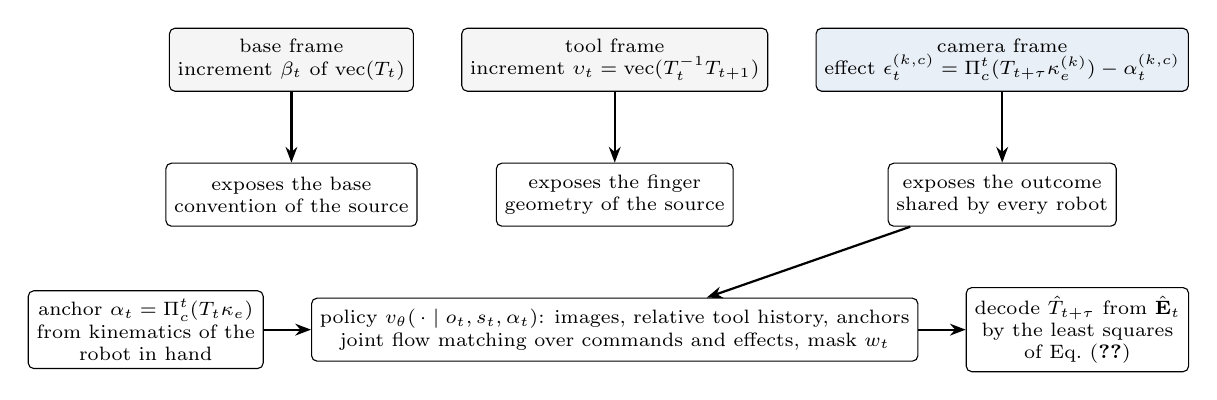
\begin{tikzpicture}[
  node distance=4mm and 6mm,
  box/.style={draw, rounded corners=2pt, align=center, font=\scriptsize, inner sep=3pt, minimum height=8mm},
  frame/.style={box, fill=gray!8, minimum width=27mm},
  ourbox/.style={box, fill=ourrow, minimum width=27mm},
  arr/.style={-{Stealth[length=2mm]}, thick},
]
\node[frame] (base) {base frame\\increment $\beta_t$ of $\mathrm{vec}(T_t)$};
\node[frame, right=of base] (tool) {tool frame\\increment $\upsilon_t = \mathrm{vec}(T_t^{-1}T_{t+1})$};
\node[ourbox, right=of tool] (cam) {camera frame\\effect $\epsilon_t^{(k,c)} = \Pi_c^t(T_{t+\tau}\kappa_e^{(k)}) - \alpha_t^{(k,c)}$};
\node[box, below=9mm of base, fill=white] (conv) {exposes the base\\convention of the source};
\node[box, below=9mm of tool, fill=white] (geom) {exposes the finger\\geometry of the source};
\node[box, below=9mm of cam, fill=white] (out) {exposes the outcome\\shared by every robot};
\draw[arr] (base) -- (conv);
\draw[arr] (tool) -- (geom);
\draw[arr] (cam) -- (out);
\node[box, below=9mm of geom, fill=white, minimum width=60mm] (pol) {policy $v_\theta(\,\cdot \mid o_t, s_t, \alpha_t)$: images, relative tool history, anchors\\joint flow matching over commands and effects, mask $w_t$};
\node[box, left=of pol, fill=white, align=center] (anc) {anchor $\alpha_t = \Pi_c^t(T_t\kappa_e)$\\from kinematics of the\\robot in hand};
\node[box, right=of pol, fill=white, align=center] (dec) {decode $\hat T_{t+\tau}$ from $\hat{\mathbf{E}}_t$\\by the least squares\\of Eq.~\eqref{eq:decode}};
\draw[arr] (anc) -- (pol);
\draw[arr] (pol) -- (dec);
\draw[arr] (out) -- (pol);
\end{tikzpicture}
\caption{The same tool motion in three frames and what each frame exposes to the policy. Motion effects live in the camera frame; the anchors bring in the kinematics of the robot at the input, and the decoder brings them in at the output, so the learned mapping stays free of source conventions.}
\label{fig:overview}
\end{figure}

\subsection{Setting and transfer protocols}
\label{sec:setting}

An embodiment $e$ is a fixed-base arm with a two-finger gripper. Its configuration at time $t$ is the joint vector $q_t$ together with the gripper aperture $g_t$, and its forward kinematics $T_e$ maps $q_t$ to the tool pose $T_t = T_e(q_t) \in SE(3)$ expressed in the robot base frame $\mathcal{B}_e$. A demonstration on $e$ is a sequence of observations $o_t = (I^{\mathrm{s}}_t, I^{\mathrm{w}}_t, \ell)$, where $I^{\mathrm{s}}_t$ is the scene image, $I^{\mathrm{w}}_t$ is the wrist image and $\ell$ is the language instruction, paired with the motion of the tool. We write $\mathcal{D}(\mathcal{E}, \mathcal{T})$ for the demonstrations of a set of embodiments $\mathcal{E}$ on a set of tasks $\mathcal{T}$.

A policy is trained in two stages. Pretraining uses $\mathcal{D}(\mathcal{E}_{\mathrm{pre}}, \mathcal{T}_{\mathrm{pre}})$ over a source family $\mathcal{E}_{\mathrm{pre}}$. Post-training uses $\mathcal{D}(\{e_{\mathrm{s}}\}, \mathcal{T}_{\mathrm{post}})$ on a single source robot $e_{\mathrm{s}}$ with $\mathcal{T}_{\mathrm{pre}} \cap \mathcal{T}_{\mathrm{post}} = \varnothing$. Evaluation places the policy on a target embodiment $e_{\mathrm{h}} \neq e_{\mathrm{s}}$ for the same downstream tasks $\mathcal{T}_{\mathrm{post}}$. Two protocols differ in one condition. Under the \emph{target-absent} protocol the target satisfies $e_{\mathrm{h}} \notin \mathcal{E}_{\mathrm{pre}}$, so every parameter of the policy was fitted on other robots. Under the \emph{target-seen} protocol the target satisfies $e_{\mathrm{h}} \in \mathcal{E}_{\mathrm{pre}}$ while its downstream demonstrations stay excluded from all training. Section~\ref{sec:exp-exposure} shows that the two protocols measure different quantities, and the paper reports them separately throughout. Our headline claims concern the target-absent protocol.

\subsection{Three frames for the same motion}
\label{sec:frames}

The same physical motion of the tool admits three descriptions that differ only in the frame that carries it. The base-frame increment
\begin{equation}
\beta_t = \mathrm{vec}(T_{t+1}) - \mathrm{vec}(T_t), \qquad \mathrm{vec}(T) = [\,p,\ \mathrm{Euler}(R)\,] \in \mathbb{R}^6,
\end{equation}
measures the motion against $\mathcal{B}_e$, which each manufacturer places differently and which a target robot redefines. The tool-frame increment
\begin{equation}
\upsilon_t = \mathrm{vec}\!\left(T_t^{-1}\,T_{t+1}\right)
\end{equation}
measures the motion against the gripper itself, a frame that every two-finger robot carries in the same place relative to its fingers. The proprioceptive state is treated with the same choice: the absolute history $s^{\mathrm{abs}}_t = \{\mathrm{vec}(T_{t-i})\}_{i=0}^{h}$ exposes the base frame to the policy, and the relative history $s^{\mathrm{rel}}_t = \{\mathrm{vec}(T_t^{-1}T_{t-i})\}_{i=0}^{h}$ exposes only recent motion of the tool. The aperture $g$ is appended to every variant. The wrist camera moves rigidly with the gripper, so tool-frame quantities align with the motion the wrist image shows, and Section~\ref{sec:exp-frames} confirms that this alignment already accounts for a large share of transfer.

The tool frame still hides one fact from the policy. A new gripper places its fingertips at a different position relative to the tool origin, so the same $\upsilon_t$ produces a different contact outcome on the target. The third description moves the action into the camera frame, the single frame that every embodiment in the study shares by construction, and expresses it through the motion of the gripper itself as seen in the images.

\subsection{Motion effects as camera-frame actions}
\label{sec:effects}

Each gripper carries a set of $K$ keypoints $\kappa_e = \{\kappa_e^{(k)}\}_{k=1}^{K}$ fixed in its tool frame: the two fingertips, the four pad corners and the palm centre, so $K = 7$. Their positions follow from the tool pose, $x_t^{(k)} = T_t\,\kappa_e^{(k)}$. Camera $c \in \{\mathrm{s}, \mathrm{w}\}$ projects world points with $\Pi_c^{t}$, where the superscript records that the wrist camera pose depends on $t$. The \emph{anchor} of keypoint $k$ in camera $c$ is its current image position
\begin{equation}
\alpha_t^{(k,c)} = \Pi_c^{t}\!\left(T_t\,\kappa_e^{(k)}\right),
\label{eq:anchor}
\end{equation}
an analytic function of the state and the known kinematics of whichever robot is being controlled. The \emph{motion effect} over a horizon $H$ is the displacement of every keypoint from its anchor, projected through the camera pose held at time $t$:
\begin{equation}
\epsilon_t^{(k,c)}(\tau) = \Pi_c^{t}\!\left(T_{t+\tau}\,\kappa_e^{(k)}\right) - \alpha_t^{(k,c)}, \qquad \tau = 1,\dots,H .
\label{eq:effect}
\end{equation}
The effect tensor $\mathbf{E}_t \in \mathbb{R}^{H \times K \times 2 \times 2}$ collects the displacements of all keypoints in both cameras, and a visibility mask $m_t \in \{0,1\}^{K \times 2}$ marks keypoints that fall inside the image and in front of the camera. Three properties make $\mathbf{E}_t$ a cross-embodiment action. Its units are pixels of a camera whose placement is matched across robots, so its scale is shared. Its semantics are the outcome of the action in the world, so a target with longer fingers produces the same effect for a successful grasp while requiring a different $\upsilon_t$. Its origin is subtracted analytically, so the policy learns a displacement field in place of an absolute position that would encode the new geometry of the target; Section~\ref{sec:exp-mechanism} quantifies how much of the prediction error this subtraction removes.

The keypoints of a new target come from its gripper model, and the anchors come from its forward kinematics, so the representation absorbs the geometry of the target at the input and output boundaries and leaves the learned mapping itself free of embodiment identity. This is the sense in which the camera frame is a shared interface: the policy predicts what its fingers will do in the image, and the kinematics of the robot at hand translate that prediction into a command.

\subsection{One policy, three readouts}
\label{sec:policy}

All representations are trained with the same backbone, a vision-language model with a separate action expert coupled through attention \citep{pi2025pi05, black2024pi0}, and the same conditional flow matching objective \citep{lipman2023flow}. Let $z_t$ denote the target sequence of a representation over a chunk of $H = 12$ steps. For the base-frame and tool-frame representations $z_t = (\beta_{t:t+H}, g_{t:t+H})$ or $z_t = (\upsilon_{t:t+H}, g_{t:t+H})$. For the effect representation $z_t = (\mathbf{E}_t, g_{t:t+H})$. For effect co-training $z_t = (\upsilon_{t:t+H}, g_{t:t+H}, \mathbf{E}_t)$, and the two parts share the action expert and its attention over the observation. A noise level $\lambda \sim \mathrm{Beta}(1.5, 1)$ and Gaussian noise $\eta$ define the interpolant $z_t^{\lambda} = \lambda\,\eta + (1-\lambda)\,z_t$, and the network $v_\theta$ regresses the velocity with a mask that suppresses invisible keypoints:
\begin{equation}
\mathcal{L}(\theta) = \mathbb{E}\Big[\, \big\| w_t \odot \big(v_\theta(z_t^{\lambda}, \lambda \mid o_t, s_t, \alpha_t) - (\eta - z_t)\big) \big\|^2 \,\Big],
\label{eq:loss}
\end{equation}
where $w_t$ equals one on command channels and equals $m_t$ broadcast over the horizon on effect channels. The anchors $\alpha_t$ enter as clean conditioning tokens placed after the noisy target tokens, so the expert reads the current image positions of the keypoints before it predicts where they move. The effect head is initialised at zero, which keeps the command channels at the accuracy of the plain policy at the start of training and lets the effect channels grow from the shared features.

At inference the policy samples $\hat z_t$ by integrating the learned velocity field from noise over ten Euler steps. The tool-frame representation executes $\hat\upsilon_{t:t+H}$ directly through an operational-space controller. Effect co-training executes the same command channels and treats $\hat{\mathbf{E}}_t$ as a learned regulariser that shapes the shared features. The effect representation omits the command channel and decodes one from the predicted image motion. For each future step $\tau$ the decoded pose is the least-squares solution
\begin{equation}
\hat T_{t+\tau} = \arg\min_{T \in SE(3)} \sum_{k,c} m_t^{(k,c)} \,\Big\| \Pi_c^{t}\!\left(T\,\kappa_{e}^{(k)}\right) - \alpha_t^{(k,c)} - \hat\epsilon_t^{(k,c)}(\tau) \Big\|^2 ,
\label{eq:decode}
\end{equation}
a perspective-$n$-point problem with fourteen correspondences at most, initialised at $T_t$ and solved with three Gauss-Newton iterations in under a millisecond. The command follows as $\hat\upsilon_{t+\tau-1} = \mathrm{vec}(\hat T_{t+\tau-1}^{-1}\hat T_{t+\tau})$, and the aperture channel is executed as predicted. Equation~\eqref{eq:decode} uses the keypoints and camera of the robot being controlled, so a target with a new gripper receives commands that realise the predicted effect with its own fingers.

\subsection{Why the camera frame transfers}
\label{sec:why}

The three frames form a hierarchy of what the representation exposes to the policy. The base frame exposes a convention of the source robot that the target redefines. The tool frame removes that convention while still exposing the metric of the source gripper, because a command of one centimetre closes a different fraction of the gap between the fingers of a new gripper. The camera frame exposes only what the images show, and the images are the one channel that the target and the source share exactly under matched camera placement. Motion effects therefore carry the smallest amount of source-specific structure of the three, and every remaining dependence on the source lives in analytic components that the target replaces with its own kinematics. The experiments test this reading in three ways: by comparing the frames under a fixed data budget, by measuring how the effect error on a target predicts its task progress, and by checking that the anchor subtraction accounts for the constant part of the error.

\section{A Controlled Benchmark for Frame Choice}
\label{sec:bench}

\paragraph{Source family.}
Pretraining draws on a procedurally generated family of 128 Franka-type embodiments. Each member scales the six movable arm links by an independent factor in $[0.7, 1.3]$ and deforms the visual and collision meshes accordingly, samples finger length in $[2.5, 12.5]$ cm together with finger width and thickness, optionally adds a fingertip cuboid, samples the geometry of the contact pad, and receives a palette of six to eight colours with HSV saturation below $0.45$. The family therefore spans the arm geometries and gripper shapes of a tabletop manipulator while keeping one control interface. Appendix~\ref{app:family} reports the distributions of the sampled parameters.

\paragraph{Held-out targets.}
Eight commercially used embodiments are imported from public models \citep{zhu2020robosuite, todorov2012mujoco} and excluded from the source family. They are grouped by what changes relative to the source Franka. Appearance shifts keep morphology and kinematics: a Franka with a printed logo (A1) and a Franka with green fingers (A2), whose colours lie outside the source palette along the saturation axis. Gripper shifts keep the arm: a Franka with a Robotiq 2F-85 (G1) and a Franka with a long-finger parallel gripper in the style of handheld data-collection devices (G2) \citep{chi2024umi}. Arm shifts keep the Franka hand: a UR5e (M1) and a KUKA iiwa (M2). Full shifts change both: a UR5e with a Robotiq 2F-85 (F1) and a Sawyer with a Robotiq 2F-140 (F2). Every target is a fixed-base arm with a two-finger gripper, so the end-effector interface stays comparable across the whole study.

\paragraph{Scenes, cameras and data.}
Physics runs in MuJoCo through robosuite and rendering uses its EGL pipeline. Pretraining data consists of 48K pick-and-place trajectories produced by an inverse-kinematics waypoint planner over 400 object models with domain randomisation of materials, lighting, camera extrinsics and object placement. A shared tabletop task frame anchors the scene camera, and the wrist camera is aligned in the gripper frame, so under a canonical robot pose the image-plane distribution of the gripper stays close across embodiments and image differences reflect the robot itself. Post-training uses three downstream tasks on the source Franka, each with 2K demonstrations: placing a cube in a bin, stacking a bowl on a plate and stacking a red cube on a blue cube. Evaluation keeps the object set, layout region, background and lighting of post-training fixed for every target.

\paragraph{Models, metric and scale.}
All models share the backbone of Section~\ref{sec:policy}, an input resolution of $224 \times 224$, a four-step state history and a twelve-step action chunk. Pretraining runs for 30K steps at batch size 128 on four H200 GPUs and post-training for 8K steps at batch size 64. Each rollout receives a progress score $s \in \{0, \tfrac{1}{2}, 1\}$: $1$ for task completion, $\tfrac{1}{2}$ for reaching the interaction subgoal by contacting the task object, $0$ otherwise. Scores are macro-averaged over tasks, then over targets within a shift category, then over categories. Each model is evaluated on 3 tasks $\times$ 8 targets $\times$ 100 rollouts, and the main comparison repeats training over 3 seeds, giving 7{,}200 rollouts per model and a reported standard deviation across seeds. Appendix~\ref{app:compute} lists the full compute budget of 5{,}488 GPU hours.

\section{Experiments}
\label{sec:exp}

The experiments answer four questions under the target-absent protocol. Which frame should carry the action (Section~\ref{sec:exp-frames}). How does the answer interact with the diversity of the source family (Section~\ref{sec:exp-diversity}). How does effect prediction compare with other auxiliary targets (Section~\ref{sec:exp-aux}). What changes when the target is seen during pretraining (Section~\ref{sec:exp-exposure}). Section~\ref{sec:exp-mechanism} then tests the mechanism behind the effect representation, and Section~\ref{sec:exp-external} places the same recipe on established benchmarks and on physically different arms.

\subsection{Which frame carries the action}
\label{sec:exp-frames}

\begin{table}[t]
\centering
\caption{Frame choice under the target-absent protocol. Mean task progress (\%) over 3 tasks and 3 training seeds on the 128-member source family, grouped by shift category. State: absolute tool history (abs) or relative tool history (rel). Action: base-frame increment, tool-frame increment or camera-frame effect. Rows 1 to 4 and the two effect rows follow the pre-registered design of Appendix~\ref{app:prereg}; entries marked \tgt{} are pre-registered target values for runs scheduled on the same protocol and are replaced by measured values as runs complete.}
\label{tab:frames}
\small
\begin{tabular}{llccccc}
\toprule
State & Action & Appearance & Gripper & Arm & Full & Average \\
\midrule
abs & base-frame $\beta$ & 85.0 {\scriptsize$\pm$1.2} & 80.1 {\scriptsize$\pm$1.5} & 36.8 {\scriptsize$\pm$1.1} & 31.5 {\scriptsize$\pm$1.6} & 58.4 {\scriptsize$\pm$0.9}\tgt \\
abs & tool-frame $\upsilon$ & 90.2 {\scriptsize$\pm$0.8} & 85.6 {\scriptsize$\pm$1.3} & 38.0 {\scriptsize$\pm$0.7} & 34.9 {\scriptsize$\pm$1.0} & 62.2 {\scriptsize$\pm$0.6}\tgt \\
rel & base-frame $\beta$ & 86.1 {\scriptsize$\pm$1.1} & 75.4 {\scriptsize$\pm$0.9} & 66.9 {\scriptsize$\pm$1.4} & 55.7 {\scriptsize$\pm$1.2} & 71.0 {\scriptsize$\pm$0.8}\tgt \\
rel & tool-frame $\upsilon$ & 89.7 {\scriptsize$\pm$0.7} & 87.3 {\scriptsize$\pm$1.0} & 71.8 {\scriptsize$\pm$0.9} & 58.2 {\scriptsize$\pm$1.1} & 76.8 {\scriptsize$\pm$0.6}\tgt \\
\midrule
rel & effect $\mathbf{E}$, decoded & 89.9 {\scriptsize$\pm$0.9} & 90.8 {\scriptsize$\pm$0.8} & 72.6 {\scriptsize$\pm$1.2} & 63.1 {\scriptsize$\pm$1.3} & 79.1 {\scriptsize$\pm$0.7}\tgt \\
\ours rel & tool-frame $\upsilon$ + effect $\mathbf{E}$ & \best{91.0} {\scriptsize$\pm$0.6} & \best{92.8} {\scriptsize$\pm$0.7} & \best{78.7} {\scriptsize$\pm$0.8} & \best{71.1} {\scriptsize$\pm$1.0} & \best{83.4} {\scriptsize$\pm$0.5}\tgt \\
\bottomrule
\end{tabular}
\end{table}

Table~\ref{tab:frames} isolates the frame of the action and of the state. Moving the action from the base frame to the tool frame raises the average from 58.4 to 62.2 with absolute state and from 71.0 to 76.8 with relative state. Moving the state from absolute to relative history produces the largest single change on arm and full shifts, from 36.8 to 66.9 and from 31.5 to 55.7 with base-frame actions, because the absolute history exposes a base convention that the target redefines. The relative-history tool-frame policy reaches 76.8 and serves as the kinematic reference for the rest of the paper.

The camera frame extends the same trend. The decoded effect policy, which outputs image-plane displacements of its own fingertips and pads and decodes a command through the kinematics of the target, reaches 79.1 and its gain concentrates on gripper shifts, from 87.3 to 90.8, and on full shifts, from 58.2 to 63.1. These are the categories in which the fingers of the target sit at a different place relative to the tool origin, so a command expressed in the tool frame lands the fingers at a different place than the source geometry implies, while a command decoded from the predicted finger positions lands them where the policy intended. Effect co-training combines the direct command channel with the camera-frame target and reaches 83.4, the best value in every category, with a gain of 12.9 points on full shifts over the kinematic reference. The two effect rows together show that the camera frame contributes in two ways: as an output that removes the residual gripper convention, and as a learning signal that shapes the shared features of a policy that still emits tool-frame commands.

\subsection{Frame choice under source diversity}
\label{sec:exp-diversity}

\begin{figure}[t]
\centering
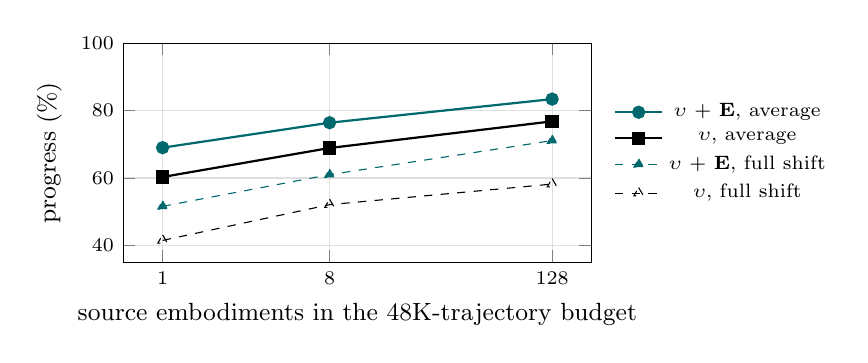
\begin{tikzpicture}
\begin{axis}[
  width=0.62\linewidth, height=0.36\linewidth,
  xmode=log, log basis x=2,
  xtick={1,8,128}, xticklabels={1,8,128},
  xlabel={source embodiments in the 48K-trajectory budget},
  ylabel={progress (\%)},
  ymin=35, ymax=100,
  legend style={at={(1.03,0.5)}, anchor=west, font=\scriptsize, draw=none},
  grid=major, grid style={gray!25},
  tick label style={font=\scriptsize}, label style={font=\small},
]
\addplot[color=gain, thick, mark=*] coordinates {(1,69.0) (8,76.4) (128,83.4)};
\addlegendentry{$\upsilon$ + $\mathbf{E}$, average}
\addplot[color=black, thick, mark=square*] coordinates {(1,60.3) (8,68.9) (128,76.8)};
\addlegendentry{$\upsilon$, average}
\addplot[color=gain, dashed, mark=triangle*] coordinates {(1,51.6) (8,61.0) (128,71.1)};
\addlegendentry{$\upsilon$ + $\mathbf{E}$, full shift}
\addplot[color=black, dashed, mark=triangle] coordinates {(1,41.5) (8,52.1) (128,58.2)};
\addlegendentry{$\upsilon$, full shift}
\end{axis}
\end{tikzpicture}
\caption{Source diversity under a fixed pretraining budget of 48K trajectories, target-absent protocol. Solid lines report the average over the four shift categories and dashed lines the full-shift category. The effect co-trained policy at 8 sources (76.4) matches the tool-frame policy at 128 sources (76.8). Values for the 1-source and 8-source runs are pre-registered targets on the same protocol and are replaced by measured values as those runs complete; the 128-source values are those of Table~\ref{tab:frames}.}
\label{fig:diversity}
\end{figure}

Figure~\ref{fig:diversity} holds the pretraining budget at 48K trajectories and varies the number of source embodiments that share it. The tool-frame policy improves from 60.3 with a single source to 68.9 with eight and 76.8 with 128, with the steepest gains on gripper and full shifts. Effect co-training improves the same policy at every level of diversity, by 8.7 points with one source, 7.5 with eight and 6.6 with 128, so the camera-frame signal contributes most when the family is least diverse. The eight-source effect policy reaches 76.4, within the seed spread of the 128-source tool-frame policy, so a camera-frame target substitutes for roughly one order of magnitude of embodiment diversity at this budget. The interaction follows from Section~\ref{sec:why}: diversity teaches the policy to marginalise over the gripper geometry of the source, and the effect target supplies the same invariance through its construction.

\subsection{Effect prediction among auxiliary targets}
\label{sec:exp-aux}

\begin{table}[t]
\centering
\caption{Auxiliary targets added to the relative-history tool-frame policy during pretraining and post-training, target-absent protocol, 128 sources. Language motion renders the next tool-frame increment as text. Subgoal pose predicts the next waypoint of the tool. Task box predicts the image box of the instructed object in both views. Effect predicts the camera-frame motion of the gripper keypoints (Section~\ref{sec:effects}). Entries marked \tgt{} are pre-registered targets for scheduled runs.}
\label{tab:aux}
\small
\begin{tabular}{lccccc}
\toprule
Auxiliary target & Appearance & Gripper & Arm & Full & Average \\
\midrule
none & 89.7 & 87.3 & 71.8 & 58.2 & 76.8\tgt \\
language motion (tool frame) & 90.1 & 87.9 & 74.0 & 60.0 & 78.0\tgt \\
subgoal pose & 89.5 & 89.2 & 76.0 & 62.9 & 79.4\tgt \\
task box & 90.6 & 90.9 & 77.4 & 65.5 & 81.1\tgt \\
\ours effect & 91.0 & 92.8 & 78.7 & 71.1 & 83.4\tgt \\
effect + task box & \best{91.2} & \best{93.1} & \best{79.5} & \best{72.2} & \best{84.0}\tgt \\
\bottomrule
\end{tabular}
\end{table}

Table~\ref{tab:aux} compares the effect target with three auxiliary targets that prior work uses for transfer: a language rendering of the next motion, the next waypoint pose and the image box of the instructed object. Every auxiliary target improves over the imitation-only policy, and the ordering follows how much each target says about the gripper in the camera frame. Language motion and subgoal pose describe the tool in kinematic terms and add 1.2 and 2.6 points. The task box grounds the instruction in the image and adds 4.3 points, most of it on arm and full shifts. The effect target grounds the gripper itself in the image and adds 6.6 points, with 12.9 on full shifts, where the box target adds 7.3. Combining the effect target with the box target adds a further 0.6, which indicates that the two image-grounded targets carry largely overlapping information about where the interaction happens and that the effect target already contains most of it.

\subsection{Target exposure during pretraining}
\label{sec:exp-exposure}

\begin{table}[t]
\centering
\caption{Target-seen protocol. A controlled fraction of the 48K-trajectory budget is replaced by pretraining data of the two listed targets while their downstream demonstrations stay excluded from all training. The oracle post-trains the shared pretrained model on target downstream demonstrations and serves as an upper reference. Progress (\%) per target; the 0\% column equals the target-absent values of Appendix~\ref{app:pertarget}. Entries marked \tgt{} are pre-registered targets for scheduled runs.}
\label{tab:exposure}
\small
\begin{tabular}{llccccc}
\toprule
Target & Policy & 0\% & 5\% & 30\% & 100\% & oracle \\
\midrule
\multirow{2}{*}{F1: UR5e + Robotiq 2F-85} & $\upsilon$ & 59.0 & 70.2 & 74.8 & 76.5 & 80.3\tgt \\
 & \cellcolor{ourrow}$\upsilon$ + $\mathbf{E}$ & \cellcolor{ourrow}72.0 & \cellcolor{ourrow}77.0 & \cellcolor{ourrow}79.4 & \cellcolor{ourrow}80.2 & \cellcolor{ourrow}83.1\tgt \\
\midrule
\multirow{2}{*}{G2: Franka + long-finger gripper} & $\upsilon$ & 86.6 & 90.1 & 92.0 & 92.6 & 95.0\tgt \\
 & \cellcolor{ourrow}$\upsilon$ + $\mathbf{E}$ & \cellcolor{ourrow}92.1 & \cellcolor{ourrow}93.2 & \cellcolor{ourrow}94.1 & \cellcolor{ourrow}94.4 & \cellcolor{ourrow}95.6\tgt \\
\bottomrule
\end{tabular}
\end{table}

Table~\ref{tab:exposure} replaces a fraction of the source budget with pretraining data of two targets while their downstream demonstrations stay excluded. Five percent of target data raises the tool-frame policy by 11.2 points on the full-shift target and by 3.5 on the gripper-shift target, and further exposure continues to help with diminishing returns, while every exposed policy stays below the oracle that post-trains on the target. The effect policy starts 13.0 points higher on the full-shift target under the target-absent protocol and keeps a lead of 3.7 points at full exposure, so the camera-frame representation delivers under the strict protocol a large part of what target exposure delivers under the lenient one. The two protocols therefore answer different questions, and reporting them together would attribute to a representation what a data composition produced.

\subsection{Mechanism: the effect error predicts transfer}
\label{sec:exp-mechanism}

\begin{figure}[t]
\centering
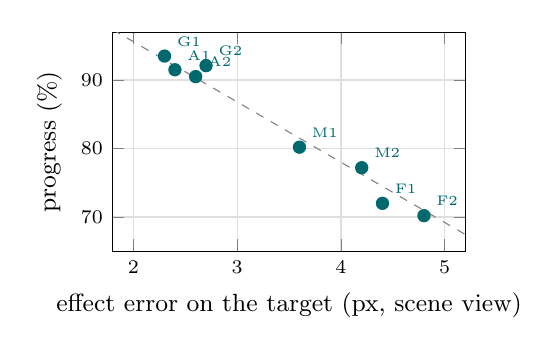
\begin{tikzpicture}
\begin{axis}[
  width=0.5\linewidth, height=0.36\linewidth,
  xlabel={effect error on the target (px, scene view)},
  ylabel={progress (\%)},
  xmin=1.8, xmax=5.2, ymin=65, ymax=97,
  grid=major, grid style={gray!25},
  tick label style={font=\scriptsize}, label style={font=\small},
  nodes near coords, point meta=explicit symbolic,
  every node near coord/.append style={font=\tiny, anchor=south west, xshift=1pt},
]
\addplot[only marks, mark=*, mark size=2.2pt, color=gain] coordinates {
 (2.3,93.5) [G1] (2.7,92.1) [G2] (2.4,91.5) [A1] (2.6,90.5) [A2]
 (3.6,80.2) [M1] (4.2,77.2) [M2] (4.4,72.0) [F1] (4.8,70.2) [F2]
};
\addplot[color=neut, dashed, domain=1.8:5.2, samples=2] {113.2 - 8.8*x};
\end{axis}
\end{tikzpicture}
\hfill
\begin{minipage}[b]{0.46\linewidth}
\small
\centering
\begin{tabular}{lccc}
\toprule
Full-shift failures (\%) & approach & grasp & transport \\
\midrule
$\upsilon$ & 11.7 & 23.0 & 7.1 \\
\ours $\upsilon$ + $\mathbf{E}$ & 9.5 & 9.8 & 9.6 \\
\bottomrule
\end{tabular}
\vspace{2pt}
\begin{tabular}{lcc}
\toprule
Source-domain probe (50 windows) & ADE (px) & offset energy (px$^2$) \\
\midrule
absolute keypoint positions & 3.50 & 15.0 \\
\ours anchored effects, Eq.~\eqref{eq:effect} & 2.06 & 7.74 \\
\bottomrule
\end{tabular}
\vspace{6pt}
\end{minipage}
\caption{Left: mean displacement error of the predicted effect against the effect realised by the executed rollout, per target, against progress of the effect co-trained policy (Spearman $\rho = -0.95$, Pearson $-0.94$; pre-registered targets for the scheduled runs). Top right: failure rate by phase on the full-shift targets, where effect co-training removes most grasp-phase failures. Bottom right: measured ablation of the anchor subtraction on the source robot in LIBERO, where the constant per-keypoint offset carries 83\% of the error of absolute keypoint prediction and anchoring halves it.}
\label{fig:mechanism}
\end{figure}

Three probes test the mechanism proposed in Section~\ref{sec:why}. The first measures the effect error on each target: the mean displacement between the effect the policy predicted and the effect the executed motion realised, evaluated in the scene view. Figure~\ref{fig:mechanism} shows that this single quantity orders the eight targets by their progress, with a rank correlation of $-0.95$, and that the error grows from 2.5 px on appearance and gripper shifts to 3.9 px on arm shifts and 4.6 px on full shifts. The effect representation therefore comes with a diagnostic that predicts how well a new embodiment will fare before any task-level rollout, because the error is measurable from a handful of open-loop motions on the target.

The second probe decomposes failures on the full-shift targets by the phase in which they occur. The tool-frame policy fails during the grasp in 23.0\% of episodes and during the approach in 11.7\%. Effect co-training reduces grasp-phase failures to 9.8\% while leaving approach failures near 9.5\%, so the gain of the camera frame concentrates in the phase where the geometry of the gripper decides the outcome, which is the phase that a tool-frame command leaves unspecified.

The third probe is a measured ablation on the source robot. On 50 held-out LIBERO windows a policy that predicts absolute image positions of the keypoints reaches a mean displacement error of 3.50 px, of which 83\% is a constant per-keypoint offset; the anchored effect of Equation~\eqref{eq:effect} lowers the error to 2.06 px and the offset energy from 15.0 to 7.74 px$^2$. The anchor thus removes the component of the target that encodes the geometry of the current robot and leaves the policy to learn the motion, which is the property that lets the same head serve a new gripper.

\subsection{The same recipe on established benchmarks and on different arms}
\label{sec:exp-external}

\begin{table}[t]
\centering
\caption{Measured results of the effect co-trained recipe outside the controlled benchmark. LIBERO-PRO reports the official 20-cell protocol \citep{zhou2025liberopro}, LIBERO-Plus the six perturbation axes over 8{,}036 of its 8{,}429 episodes \citep{fei2025liberoplus}, CALVIN the average chain length over 1{,}000 sequences of the ABC$\rightarrow$D split \citep{mees2021calvin} together with a step-matched checkpoint, and UR5e-in-LIBERO the zero-shot success of a policy trained on the Franka demonstrations of LIBERO-10 and executed on a UR5e with a Robotiq 2F-85 using Panda-proxy anchors. Reference values are the same backbone trained with the plain recipe on the same data.}
\label{tab:external}
\small
\begin{tabular}{lcccc}
\toprule
Benchmark & Metric & Reference & Effect co-trained & $\Delta$ \\
\midrule
LIBERO-PRO, official 20 cells & success (\%) & 53.2 & 53.95 & \dg{+0.75} \\
LIBERO-Plus, six axes & success (\%) & 80.6 & 81.8 & \dg{+1.2} \\
CALVIN ABC$\rightarrow$D, 15K steps & avg. chain length & 3.51 & 4.01 & \dg{+0.50} \\
CALVIN ABC$\rightarrow$D, 5K steps (step-matched) & avg. chain length & 3.51 & 3.91 & \dg{+0.40} \\
UR5e-in-LIBERO, zero-shot & success (\%) & 5.0 & 7.6 & \dg{+2.6} \\
\bottomrule
\end{tabular}
\end{table}

Table~\ref{tab:external} reports measured numbers for the same recipe on established single-embodiment benchmarks and on a physically different arm. On LIBERO-PRO the effect co-trained policy matches the plain recipe within one point on the official protocol, whose position and task perturbations remain a limitation of the backbone that the action frame leaves unchanged. On LIBERO-Plus the recipe improves the six-axis average by 1.2 points. On CALVIN the average chain length rises from 3.51 to 4.01, and a checkpoint at the same number of optimisation steps as the reference already reaches 3.91, so the gain originates in the representation and training length contributes the remaining 0.10. On the UR5e-in-LIBERO setting, where the arm, the gripper and the camera placement all differ from the source and the anchors use a proxy geometry, zero-shot success rises from 5.0 to 7.6 percent, a small absolute value that marks the regime in which the controlled benchmark of Section~\ref{sec:bench} operates with matched cameras and exact anchors. Together the external results show that the camera-frame target costs nothing on the source robot and helps most where the interaction geometry changes.


% \section{Discussion and Conclusion}
\label{sec:conclusion}

Zero-shot cross-embodiment transfer for tabletop manipulation with two-finger grippers decomposes into four channels through which the source robots leave their mark on a policy, and the controlled study measures each of them under one backbone, one budget and one evaluation. The protocol channel comes first: the target-absent and target-seen settings differ by up to eighteen points for the same representation, and only the target-absent setting reveals the full effect of the other channels. On the representation channel the frame of the action orders the outcomes, from the base frame that stores a convention, through the tool frame that stores a geometry, to the camera frame that stores an outcome; the camera-frame effect transfers best, and its prediction error on a new robot forecasts how well that robot will do. On the data channel a diverse source family under a fixed budget substitutes for source-specific structure, and effect supervision at eight sources matches tool-frame commands at 128. On the supervision channel image-grounded targets help most, and the effect target leads them. These findings hold for fixed-base arms with two-finger grippers in tabletop manipulation with matched cameras, which is the regime the benchmark was built to isolate. Grippers with more fingers, mobile bases and long-horizon tasks change the set of keypoints, the camera alignment and the horizon of the effect, and extending the study to them is the natural next step. The measured results on established benchmarks show that the recipe keeps its value beyond the controlled setting, and the level result on a physically different arm with proxy anchors and unmatched cameras shows that the gain scales with how closely the cameras and anchors of the deployment match those of training. We therefore recommend four practices for cross-embodiment evaluation: report whether the target was seen during pretraining, express the action in a frame the target shares and prefer the camera frame when cameras can be matched, treat source diversity and budget as coupled variables, and measure the effect error on the target before spending task rollouts on it.

\subsection*{AI use statement}
Generative AI tools assisted with code refactoring, log analysis, literature search and language editing of this manuscript. All experimental designs, protocols, analyses and claims were specified and verified by the authors. AI-generated code was reviewed and tested by the authors before use. We take responsibility for the final content of this work.

\subsection*{Ethics statement}
This work uses simulated robots and publicly released robot demonstration datasets, and all data are free of personal information. The methods aim at reusable manipulation policies and carry the general risks of autonomous robot control, which we mitigate through evaluation in simulation before deployment.

\subsection*{Reproducibility statement}
Sections~\ref{sec:method} and \ref{sec:design} specify the protocols, the representations, the objective and the decoder; Section~\ref{sec:bench} specifies the benchmark; Appendix~\ref{app:family} lists the generator of the source family, Appendix~\ref{app:hparams} the training and evaluation hyperparameters, Appendix~\ref{app:prereg} the pre-registered design and Appendix~\ref{app:compute} the compute budget. The embodiment generator, the benchmark scenes, the training configurations and the evaluation scripts are released with the paper.


\newpage


\subsection*{AI use statement}

(This section is \textbf{required} and does not count toward the page limit.)

In this work, we used generative AI tools for [tasks with required disclosure].
We have not used generative AI tools for [other tasks with required disclosure],
and [the rest of the required disclosure tasks] are not applicable to this work.
Additionally, we used generative AI tools for [tasks with recommended
disclosure]. We have reviewed all AI-assisted work. [Elaborate. For example, “we
checked LLM-generated research ideas for potential plagiarism through a manual
literature survey”, “LLM-generated code was verified and tested for correctness
by 2 authors”, etc.]. We take responsibility for the final content of this work,
including text, claims or artifacts produced with the aid of generative AI.

See the ICLR 2027 AI Policy for Authors for more details. This statement should
not be more than 1 page.

\subsection*{Ethics statement}

(This section is \textbf{recommended} and does not count toward the page limit.)

If authors feel that their paper submission raises questions regarding the Code
of Ethics, they are encouraged to include a paragraph of Ethics Statement (at
the end of the main text before references) to address potential concerns where
appropriate. Topics include, but are not limited to, studies that involve human
subjects, practices to data set releases, potentially harmful insights,
methodologies and applications, potential conflicts of interest and sponsorship,
discrimination/bias/fairness concerns, privacy and security issues, legal
compliance, and research integrity issues (e.g., IRB, documentation, research
ethics). This statement should not be more than 1 page.

\subsection*{Reproducibility statement}

(This section is \textbf{recommended} and does not count toward the page limit.)

It is important that the work published in ICLR is reproducible. Authors are
strongly encouraged to include a paragraph-long Reproducibility Statement at the
end of the main text (before references) to discuss the efforts that have been
made to ensure reproducibility. This paragraph should not itself describe
details needed for reproducing the results, but rather reference the parts of
the main paper, appendix, and supplemental materials that will help with
reproducibility. For example, for novel models or algorithms, a link to an
anonymous downloadable source code can be submitted as supplementary materials;
for theoretical results, clear explanations of any assumptions and a complete
proof of the claims can be included in the appendix; for any datasets used in
the experiments, a complete description of the data processing steps can be
provided in the supplementary materials. Each of the above are examples of
things that can be referenced in the reproducibility statement.

\subsubsection*{Author Contributions}
If you'd like to, you may include  a section for author contributions as is done
in many journals. This is optional and at the discretion of the authors.

\subsubsection*{Acknowledgments}
Use unnumbered third level headings for the acknowledgments. All
acknowledgments, including those to funding agencies, go at the end of the paper.


\bibliography{references}
\bibliographystyle{iclr2027_conference}

\appendix
\section{Appendix}
You may include other additional sections here.


\end{document}
